
Table Alias names

It is possible within a SELECT statement to use temporary labels, called aliases, for the table names; this can be a useful shorthand to reference the tables.  Single letters may be used although it is advisable to use meaningful aliases to aid readability.  Once an alias is declared for a table it must always be used throughout the query; using the table name will generate an error.

\ \ SELECT \ \ CUST.REFNO, NAME, ACC.ACCNO, BALANCE

\ \ FROM \ \ CUST  

\ \ \ \ INNER JOIN\ \ CUSTACC 

\ \ \ \ \ \ ON \ \ CUST.REFNO = CUSTACC.REFNO

\ \ \ \ INNER JOIN\ \ ACC 

\ \ \ \ \ \ ON \ \ CUSTACC.ACCNO = ACC.ACCNO ;

becomes:

\ \ SELECT \ \ C.REFNO, NAME, A.ACCNO, BALANCE

\ \ FROM \ \ CUST  C

\ \ \ \ INNER JOIN\ \ CUSTACC CA 

\ \ \ \ \ \ ON \ \ C.REFNO = CA.REFNO

\ \ \ \ INNER JOIN\ \ ACC A 

\ \ \ \ \ \ ON \ \ CA.ACCNO = A.ACCNO ;

G1\ \ Show the name and salary of every employee and the name of the department where they work. Use aliases for table names.

\begin{flushleft}
\tablefirsthead{}
\tablehead{}
\tabletail{}
\tablelasttail{}
\begin{supertabular}{|m{14.303cm}|}
\hline
\\\hline
\end{supertabular}
\end{flushleft}
Self join

Table EMP contains details of Employees.  One piece of data is the Employee Number of their manager.  How do we obtain the name of their manager?  This is a common occurrence, where a table needs to 'link back' to itself.  

We cannot do this directly, and we cannot reference two tables with the same name.  But we can have a second copy of a table which is referenced by a (sensible) alias.  If we give one copy of table EMP the alias 'Manager' (and consider it to be the list of managers), and the second 'Staff' (and consider it to be the list of staff, some of whom are also managers), we can now treat them as two separate tables.  Note that all column names are duplicated and will need to be referenced using the table.column  notation.

What is the relationship between the data in these two copies of table EMP?  (You may find it helpful to place two appropriately headed copies of the printed tables next to one another and work out who is Smith's manager).  The MGR column of the Staff table equates to the EMPNO column of the Manager table.

G2\ \ Show the name, employee number and manager's name of those who are managed by either Blake or Jones.  Carefully check your results.

\begin{flushleft}
\tablefirsthead{}
\tablehead{}
\tabletail{}
\tablelasttail{}
\begin{supertabular}{|m{14.793cm}|}
\hline
Select

From

INNER Join\ \ \ \ \ \ \ \ 

On

Where\\\hline
\end{supertabular}
\end{flushleft}
G3\ \ Display the names of all the people in a management position, their department number and the number of staff for whom they have direct responsibility.  (This is not a case of asking for those with job 'MANAGER'.  We are looking for those employees that manage one or more employees, ie where employees have them as their manager (column MGR).

\begin{flushleft}
\tablefirsthead{}
\tablehead{}
\tabletail{}
\tablelasttail{}
\begin{supertabular}{|m{14.583cm}|}
\hline
Select

From

INNER Join

ON

GROUP By

\\\hline
\end{supertabular}
\end{flushleft}
G4\ \ Show only those managers, as defined above, who are directly responsible for the management of more than two people.

\begin{flushleft}
\tablefirsthead{}
\tablehead{}
\tabletail{}
\tablelasttail{}
\begin{supertabular}{|m{14.583cm}|}
\hline
Select

From

INNER Join

ON

GROUP BY

HAVING

\\\hline
\end{supertabular}
\end{flushleft}
G5\ \ Display the employee name, location and department number of those managers, as defined in G3, whose salary is greater than £1500. 

\begin{flushleft}
\tablefirsthead{}
\tablehead{}
\tabletail{}
\tablelasttail{}
\begin{supertabular}{|m{14.793cm}|}
\hline
Select

\\\hline
\end{supertabular}
\end{flushleft}
\ \ How many rows have you selected?  Is that correct?  This problem will be looked into soon.

\section{OUTER JOIN}
G6\ \ For all employees list their name, salary and location.

\begin{flushleft}
\tablefirsthead{}
\tablehead{}
\tabletail{}
\tablelasttail{}
\begin{supertabular}{|m{14.583cm}|}
\hline
Select

FROM

INNER JOIN

ON\\\hline
Some data is missing. Which data? And Why?

\\\hline
\end{supertabular}
\end{flushleft}
G7\ \ List the names of Employees, and their manager's name.  

\begin{flushleft}
\tablefirsthead{}
\tablehead{}
\tabletail{}
\tablelasttail{}
\begin{supertabular}{|m{14.583cm}|}
\hline
Select

FROM

INNER JOIN

ON\\\hline
Which data is missing, and why?

\\\hline
\end{supertabular}
\end{flushleft}
You have produced solutions to a number of questions where the results that are produced are correct as far as they go, but not totally correct as some rows are missing (see F5).  In the Equi and Self Joins, rows are only selected where the join is satisfied, ie where matching values are found in both tables.

So an inner join displays the result on the right: Smith and Done are both in the CUST table, but no information s shown about them.

\begin{flushleft}
\tablefirsthead{}
\tablehead{}
\tabletail{}
\tablelasttail{}
\begin{supertabular}{m{7.99cm}|m{7.988cm}}
SELECT  NAME, ADDRESS, ACCNO

FROM \ \ CUST

INNER JOIN  CUSTACC

ON  CUST.REFNO  = CUSTACC.REFNO ;



\begin{center}
  
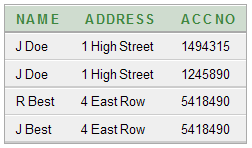
\includegraphics[width=6.685cm,height=3.916cm]{images/img (46).png}

\end{center}
 &
SELECT  NAME, ADDRESS, ACCNO

FROM \ \  CUST

LEFT OUTER JOIN  CUSTACC

ON  CUST.REFNO  = CUSTACC.REFNO ;

   
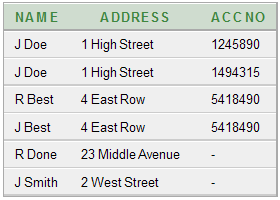
\includegraphics[width=7.392cm,height=5.308cm]{images/img (47).png}
 \\
\end{supertabular}
\end{flushleft}
To display them, we use another form of join - the OUTER JOIN - which returns rows as for the INNER JOIN but, in addition, returns extra rows: those from one table which have no match in the other table. They show us customers who don't have an account.

There are three forms of Outer Join, the LEFT OUTER JOIN, RIGHT OUTER JOIN and FULL OUTER JOIN, the correct one to use is determined by which table has the extra rows. In our example the table CUST contains the extra rows and therefore we use the join to `point at' that table: the table name 'CUST' is to the LEFT of the words OUTER JOIN.

Note that the following two formats will produce exactly the same results:

\begin{flushleft}
\tablefirsthead{}
\tablehead{}
\tabletail{}
\tablelasttail{}
\begin{supertabular}{|m{7.99cm}|m{7.988cm}|}
\hline
SELECT  NAME, ADDRESS, ACCNO

FROM  CUSTACC

RIGHT OUTER JOIN CUST

ON  CUSTACC.REFNO  = CUST.REFNO ;

 &
SELECT  NAME, ADDRESS, ACCNO

FROM  CUST

LEFT OUTER JOIN  CUSTACC

ON  CUSTACC.REFNO  = CUST.REFNO ;

\\\hline
\end{supertabular}
\end{flushleft}
If you join together three or more tables where any of the relationships are optional you must ensure that you use an outer join in each of the join statements.  Failure to do so will produce an error message saying that the join is ambiguous.

\ \ SELECT \ \ CUST.REFNO, NAME, ACC.ACCNO, BALANCE, 

\ \ \ \ \ \ BALANCE *0.03 AS INTEREST

\ \ FROM \ \ CUST

\ \ \ \ LEFT OUTER JOIN \ \ CUSTACC 

\ \ \ \ \ \ ON\ \ CUST.REFNO  =  CUSTACC.REFNO

\ \ \ \ LEFT OUTER JOIN\ \ \ \ ACC  

\ \ \ \ \ \ ON \ \ CUSTACC.ACCNO  = ACC.ACCNO;

   
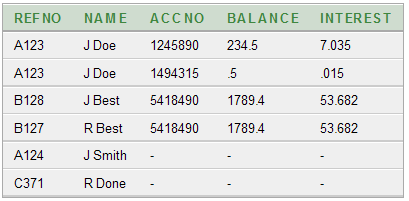
\includegraphics[width=10.843cm,height=5.345cm]{images/img (48).png}
 

Note the column titles, particularly ACCNO.  This column name exists in both the ACC and CUSTACC tables yet the display does not identify this, even though we have specified ACC.ACCNO.

The value in the ACCNO column for A124 is not zero but NULL.  It can be treated like any other value and used within Criteria (column IS NULL) - a very powerful facility.  Any calculations performed on a column containing a null value will also return a null.

\ \ SELECT \ \ CUST.REFNO, NAME, ACC.ACCNO, BALANCE, 

\ \ \ \ \ \ BALANCE *0.03 AS INTEREST

\ \ FROM \ \ CUST

\ \ \ \ LEFT OUTER JOIN \ \ CUSTACC 

\ \ \ \ \ \ ON\ \ CUST.REFNO  =  CUSTACC.REFNO

\ \ \ \ LEFT OUTER JOIN\ \ ACC  

\ \ \ \ \ \ ON \ \ CUSTACC.ACCNO  = ACC.ACCNO

\ \ WHERE\ \ ACC.ACCNO IS NULL ;

   
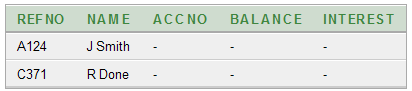
\includegraphics[width=10.918cm,height=2.388cm]{images/img (49).png}
 

G8\ \ Display the employee name, location and department name of anyone whose salary is greater than £1500.  Ensure all relevant employees are selected.

\begin{flushleft}
\tablefirsthead{}
\tablehead{}
\tabletail{}
\tablelasttail{}
\begin{supertabular}{|m{14.793cm}|}
\hline
SELECT

FROM

\_\_\_\_ OUTER JOIN

ON

WHERE

\\\hline
\end{supertabular}
\end{flushleft}
G9\ \ For all employees (i.e. to include the President) display their own name and employee number and their manager's name and number.

\ \ (Check this output very carefully against the sample tables).

\begin{flushleft}
\tablefirsthead{}
\tablehead{}
\tabletail{}
\tablelasttail{}
\begin{supertabular}{|m{14.266cm}|}
\hline
SELECT

\\\hline
\end{supertabular}
\end{flushleft}
G10\ \ List the names of all employees that are not in the RESEARCH department.  Ensure you check the results generated by your solution. Ensure you have displayed nine rows, including the President.

\begin{flushleft}
\tablefirsthead{}
\tablehead{}
\tabletail{}
\tablelasttail{}
\begin{supertabular}{|m{14.266cm}|}
\hline
SELECT

\\\hline
\end{supertabular}
\end{flushleft}
G11\ \ List the names of those departments that have no employees.

\begin{flushleft}
\tablefirsthead{}
\tablehead{}
\tabletail{}
\tablelasttail{}
\begin{supertabular}{|m{14.266cm}|}
\hline
SELECT

\\\hline
\end{supertabular}
\end{flushleft}
G12\ \ List the departmental names and number of employees in departments with fewer than 6 employees.

\begin{flushleft}
\tablefirsthead{}
\tablehead{}
\tabletail{}
\tablelasttail{}
\begin{supertabular}{|m{14.266cm}|}
\hline
SELECT

\\\hline
\end{supertabular}
\end{flushleft}
\clearpage

